\section{РУКОВОДСТВО ПОЛЬЗОВАТЕЛЯ}
\label{sec:manual}

Разработанные системные вызовы представляют собой набор патчей на языке Си, при
необходимости прикладываемых к ядру. Пользователь может как использовать готорые
примеры прикладных программ, так и пользоваться новыми системными вызовами
напрямую.

\subsection{Требования к аппаратному и программному обеспечению}

Минимальные требования для сборки и функционирования модифицированного ядра:
\begin{itemize}
\item GNU C 3.2;
\item GNU make 3.81;
\item binutils 2.20;
\item flex 2.5.35;
\item bison 2.0;
\item util-linux 2.10o;
\item module-init-tools 0.9.10;
\item e2fsprogs 1.41.4;
\item jfsutils 1.1.3;
\item reiserfsprogs 3.6.3;
\item xfsprogs 2.6.0;
\item squashfs-tools 4.0;
\item btrfs-progs 0.18;
\item pcmciautils 004;
\item quota-tools 3.09;
\item PPP 2.4.0;
\item isdn4k-utils 3.1pre1;
\item nfs-utils 1.0.5;
\item procps 3.2.0;
\item oprofile 0.9;
\item udev 081;
\item grub 0.93;
\item mcelog 0.6;
\item iptables 1.4.2;
\item openssl \& libcrypto 1.0.0;
\item bc 1.06.95;
\item XZ Utils 5.0;
\item tar 1.20;
\item QEMU 2.0 (опционально);
\item процессор совместимый с Intel i386;
\item свободное место на жестком диске 350 Мб;
\item оперативная память 512 Mб.
\end{itemize}

\subsection{Руководство по сборке и запуску программного средства}

Перед сборкой и установной ядра необходимо получить соответствующие исходные
коды, распаковав архив с необходимой версией ядра и приложив к ней патчи:

\medskip
\begin{lstlisting}[style=cstyle]
$ tar xf linux-4.14.2.tar.xz
$ cd linux-4.14.2
$ patch -p1 < pateenok.patch
$ patch -p1 < brouka.patch
\end{lstlisting}
\medskip

При необходимости можно использовать другие версии ядра, которые доступны на
сайте \texttt{https://www.kernel.org/}, что изображено на рисунке
\ref{fig:kernelorg}. Далее необходимо проконфигурировать
ядро. Одни из наиболее простых вариантов~--- использование конфигурации текущей
системы или стандартной конфигурации текущей архитектуры. При этом полезно
создать отдельную директорию для файлов сборки:

\begin{figure}
  \centering
  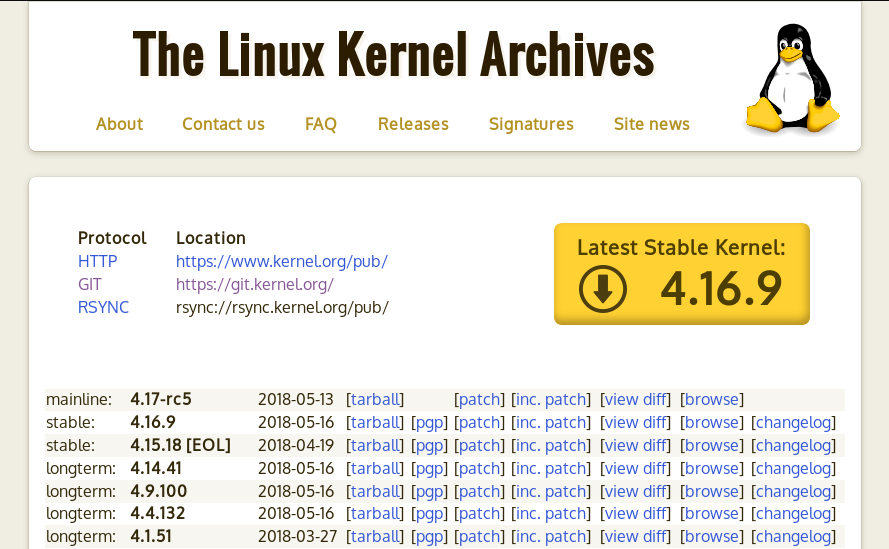
\includegraphics[width=\textwidth]{kernelorg.png}
  \caption{Получение исходных кодов ядра}
  \label{fig:kernelorg}
\end{figure}

\medskip
\begin{lstlisting}[style=cstyle]
$ mkdir ../obj/
$ cp /boot/config-$(uname -r) ../obj/.config
$ # make O=../obj defconfig
\end{lstlisting}
\medskip

Конфигурация ядра может производиться несколькими способами, при этом важно
включить параметры \texttt{CONFIG\_PIDMAP} и \texttt{CONFIG\_FDMAP}:
\begin{itemize}
\item \texttt{make O=../obj config}~--- простой текстовый интерфейс,
  спрашивающий о каждой конфигурационной опции;
\item \texttt{make O=../obj menuconfig}~--- псевдографический интерфейс на базе
  Ncurses;
\item \texttt{make O=../obj xconfig}~--- графический интерфейс на базе Qt;
\item \texttt{make O=../obj gconfig}~--- графический интерфейс на GTK+;
\item \texttt{make O=../obj oldconfig}~--- текстовый интерфейс, берет за основу
  конфигурацию в \texttt{.config}, спрашивая только о новых конфигурационных
  параметрах.
\end{itemize}

После конфигурации можно приступить к конфигурации ядра:
\medskip
\begin{lstlisting}[style=cstyle]
$ make O=../obj -j4
\end{lstlisting}
\medskip

Параметр \texttt{-j} указывает на число потоков сборки.
После установки необходимо установить ядро в систему:
\medskip
\begin{lstlisting}[style=cstyle]
$ sudo make O=../obj install
$ sudo make O=../obj modules_install
\end{lstlisting}
\medskip

Также возможно использование измененного ядра без установки, запуская его на
виртуальной машине, например, QEMU, что проще для тестирования, а также удобно
при разработке, так как ускоряет цикл перекомпиляции-запуска. Для этого сначала
нужно подготовить образ диска, который будет использоваться машиной в качестве
корневой файловой системы. Образ диска в формате RAW размеров в 1 Гб создается
следующей командой:
\medskip
\begin{lstlisting}[style=cstyle]
$ qemu-img create image.raw 1g
\end{lstlisting}
\medskip

После этого необходимо создать на диске файловую систему и смонтировать ее в
созданную директорию:
\medskip
\begin{lstlisting}[style=cstyle]
$ sudo mkfs.ext2 image.raw
$ mkdir ../mnt
$ sudo mount -o loop image.raw ../mnt
\end{lstlisting}
\medskip

Далее на созданный образ диска устанавливается система:
\medskip
\begin{lstlisting}[style=cstyle]
$ sudo debootstrap --arch amd64 jessie ../mnt
$ sudo umount ../mnt
\end{lstlisting}
\medskip

После чего виртуальну машину можно запустить, указав путь к ядру и образу диска,
следующей командой:
\medskip
\begin{lstlisting}[style=cstyle]
$ qemu-system-x86_64  -kernel arch/x86_64/boot/bzImage \
    -drive file=../image.img,index=0,media=disk,format=raw \
    -append "root=/dev/sda rw single" -enable-kvm
\end{lstlisting}
\medskip

В некоторых сборках QEMU поставляется без встроенного клиента системы VNC, в
таком случае при запуске в графическом режиме можно использовать Vinagre, по
умолчанию подключившись к порту 5900. Результат запуска показан на рисунке
\ref{fig:qemu}.

\begin{figure}
  \centering
  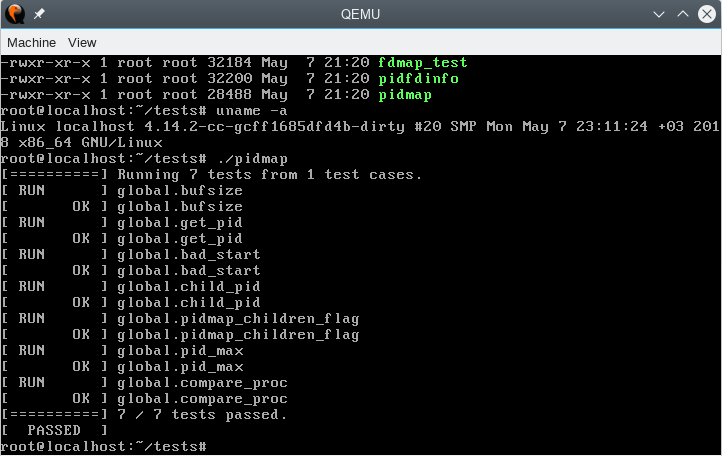
\includegraphics[width=\textwidth]{qemu.png}
  \caption{Запуск машины с пропатченным ядром в QEMU}
  \label{fig:qemu}
\end{figure}

Как уже было сказано, примеры рабочих пользовательских программ, а также
тестовые программы расположены соответственно в \texttt{samples/} и
\texttt{tools/testing/selftests/}. При желании использовать разработанные
системные вызовы в собственных программмах, использовать новые системные вызовы
можно несколькими способами.

Для большинства существующих системных вызовов Glibc предоставляет
функции-обертки, однако нашем случае по очевидным причинам готовой обертки нет.
Однако, для подобных случаев существует библиотечная функция \texttt{syscall()},
позволяющая исполнить системный вызов напрямую, используя его номер. При этом в
случае возврата вызовом ошибки Glibc самостоятельно изменит содержимое
переменной \texttt{errno}, а сама функция возвратит -1. Для использования
функции подключается заголовочный файл \texttt{unistd.h}. Номера системных
вызовов следующие:
\begin{itemize}
\item 333~--- pidfdopen;
\item 335~--- pidfdinfo;
\item 336~--- fdmap;
\item 337~--- pidmap;
\item 339~--- pidinfo.
\end{itemize}

Если ядро было установлено в систему при помощи \texttt{make install}, в
директории с системными заголовками был помещен файл \texttt{sys/syscall.h},
сгенерированный в процессе компиляции ядра и содержащий макроопределения вида
\texttt{SYS\_fdmap}, уже содержащие номера вызовов, в таком случае вызов
\texttt{pidmap()} будет выглядеть следующим образом:
\medskip
\begin{lstlisting}[style=cstyle]
long ret = syscall(SYS_pidmap, pid, pids, count, start_pid, flags);
if (ret == -1)
	perror("pidmap");
\end{lstlisting}
\medskip

Также есть возможность вызова путем ассемблерной вставки. При этом возвратится
настоящий код возврата, без искажений и записи в \texttt{errno}. При этом на
архитектуре x86\_64 регистры заполняются аргументами в следующем порядке:
\texttt{rdi}, \texttt{rsi}, \texttt{rdx}, \texttt{r10}, \texttt{r8},
\texttt{r9}. Таким образом, вызов \texttt{fdmap()} будет выглядеть следующим
образом:
\medskip
\begin{lstlisting}[style=cstyle]
register long r10 asm ("r10") = start;
register long r8 asm ("r8") = flags;
long ret;
asm volatile (
	"syscall"
	: "=a" (ret)
	: "0" (333), "D" (pid), "S" (fd),
	  "d" (nfd), "r" (r10), "r" (r8)
	: "rcx", "r11", "cc", "memory"
);
if (ret < 0)
	dprintf(2, "fdmap: error %ld", ret);
\end{lstlisting}
\medskip

Таким образом, использование реализованных системных вызовов не является сложной
задачей, достаточно иметь небольшой опыт языка Си. При этом, даже без знания Си
возможно использование разработки в виде готовых примеров программ.
